\documentclass[]{article}
\usepackage{lmodern}
\usepackage{amssymb,amsmath}
\usepackage{ifxetex,ifluatex}
\usepackage{fixltx2e} % provides \textsubscript
\ifnum 0\ifxetex 1\fi\ifluatex 1\fi=0 % if pdftex
  \usepackage[T1]{fontenc}
  \usepackage[utf8]{inputenc}
\else % if luatex or xelatex
  \ifxetex
    \usepackage{mathspec}
  \else
    \usepackage{fontspec}
  \fi
  \defaultfontfeatures{Ligatures=TeX,Scale=MatchLowercase}
\fi
% use upquote if available, for straight quotes in verbatim environments
\IfFileExists{upquote.sty}{\usepackage{upquote}}{}
% use microtype if available
\IfFileExists{microtype.sty}{%
\usepackage{microtype}
\UseMicrotypeSet[protrusion]{basicmath} % disable protrusion for tt fonts
}{}
\usepackage[margin=1in]{geometry}
\usepackage{hyperref}
\hypersetup{unicode=true,
            pdftitle={Simulating Discrete Markov Chains},
            pdfauthor={Prof.~S. Pesenti},
            pdfborder={0 0 0},
            breaklinks=true}
\urlstyle{same}  % don't use monospace font for urls
\usepackage{color}
\usepackage{fancyvrb}
\newcommand{\VerbBar}{|}
\newcommand{\VERB}{\Verb[commandchars=\\\{\}]}
\DefineVerbatimEnvironment{Highlighting}{Verbatim}{commandchars=\\\{\}}
% Add ',fontsize=\small' for more characters per line
\usepackage{framed}
\definecolor{shadecolor}{RGB}{248,248,248}
\newenvironment{Shaded}{\begin{snugshade}}{\end{snugshade}}
\newcommand{\AlertTok}[1]{\textcolor[rgb]{0.94,0.16,0.16}{#1}}
\newcommand{\AnnotationTok}[1]{\textcolor[rgb]{0.56,0.35,0.01}{\textbf{\textit{#1}}}}
\newcommand{\AttributeTok}[1]{\textcolor[rgb]{0.77,0.63,0.00}{#1}}
\newcommand{\BaseNTok}[1]{\textcolor[rgb]{0.00,0.00,0.81}{#1}}
\newcommand{\BuiltInTok}[1]{#1}
\newcommand{\CharTok}[1]{\textcolor[rgb]{0.31,0.60,0.02}{#1}}
\newcommand{\CommentTok}[1]{\textcolor[rgb]{0.56,0.35,0.01}{\textit{#1}}}
\newcommand{\CommentVarTok}[1]{\textcolor[rgb]{0.56,0.35,0.01}{\textbf{\textit{#1}}}}
\newcommand{\ConstantTok}[1]{\textcolor[rgb]{0.00,0.00,0.00}{#1}}
\newcommand{\ControlFlowTok}[1]{\textcolor[rgb]{0.13,0.29,0.53}{\textbf{#1}}}
\newcommand{\DataTypeTok}[1]{\textcolor[rgb]{0.13,0.29,0.53}{#1}}
\newcommand{\DecValTok}[1]{\textcolor[rgb]{0.00,0.00,0.81}{#1}}
\newcommand{\DocumentationTok}[1]{\textcolor[rgb]{0.56,0.35,0.01}{\textbf{\textit{#1}}}}
\newcommand{\ErrorTok}[1]{\textcolor[rgb]{0.64,0.00,0.00}{\textbf{#1}}}
\newcommand{\ExtensionTok}[1]{#1}
\newcommand{\FloatTok}[1]{\textcolor[rgb]{0.00,0.00,0.81}{#1}}
\newcommand{\FunctionTok}[1]{\textcolor[rgb]{0.00,0.00,0.00}{#1}}
\newcommand{\ImportTok}[1]{#1}
\newcommand{\InformationTok}[1]{\textcolor[rgb]{0.56,0.35,0.01}{\textbf{\textit{#1}}}}
\newcommand{\KeywordTok}[1]{\textcolor[rgb]{0.13,0.29,0.53}{\textbf{#1}}}
\newcommand{\NormalTok}[1]{#1}
\newcommand{\OperatorTok}[1]{\textcolor[rgb]{0.81,0.36,0.00}{\textbf{#1}}}
\newcommand{\OtherTok}[1]{\textcolor[rgb]{0.56,0.35,0.01}{#1}}
\newcommand{\PreprocessorTok}[1]{\textcolor[rgb]{0.56,0.35,0.01}{\textit{#1}}}
\newcommand{\RegionMarkerTok}[1]{#1}
\newcommand{\SpecialCharTok}[1]{\textcolor[rgb]{0.00,0.00,0.00}{#1}}
\newcommand{\SpecialStringTok}[1]{\textcolor[rgb]{0.31,0.60,0.02}{#1}}
\newcommand{\StringTok}[1]{\textcolor[rgb]{0.31,0.60,0.02}{#1}}
\newcommand{\VariableTok}[1]{\textcolor[rgb]{0.00,0.00,0.00}{#1}}
\newcommand{\VerbatimStringTok}[1]{\textcolor[rgb]{0.31,0.60,0.02}{#1}}
\newcommand{\WarningTok}[1]{\textcolor[rgb]{0.56,0.35,0.01}{\textbf{\textit{#1}}}}
\usepackage{graphicx,grffile}
\makeatletter
\def\maxwidth{\ifdim\Gin@nat@width>\linewidth\linewidth\else\Gin@nat@width\fi}
\def\maxheight{\ifdim\Gin@nat@height>\textheight\textheight\else\Gin@nat@height\fi}
\makeatother
% Scale images if necessary, so that they will not overflow the page
% margins by default, and it is still possible to overwrite the defaults
% using explicit options in \includegraphics[width, height, ...]{}
\setkeys{Gin}{width=\maxwidth,height=\maxheight,keepaspectratio}
\IfFileExists{parskip.sty}{%
\usepackage{parskip}
}{% else
\setlength{\parindent}{0pt}
\setlength{\parskip}{6pt plus 2pt minus 1pt}
}
\setlength{\emergencystretch}{3em}  % prevent overfull lines
\providecommand{\tightlist}{%
  \setlength{\itemsep}{0pt}\setlength{\parskip}{0pt}}
\setcounter{secnumdepth}{0}
% Redefines (sub)paragraphs to behave more like sections
\ifx\paragraph\undefined\else
\let\oldparagraph\paragraph
\renewcommand{\paragraph}[1]{\oldparagraph{#1}\mbox{}}
\fi
\ifx\subparagraph\undefined\else
\let\oldsubparagraph\subparagraph
\renewcommand{\subparagraph}[1]{\oldsubparagraph{#1}\mbox{}}
\fi

%%% Use protect on footnotes to avoid problems with footnotes in titles
\let\rmarkdownfootnote\footnote%
\def\footnote{\protect\rmarkdownfootnote}

%%% Change title format to be more compact
\usepackage{titling}

% Create subtitle command for use in maketitle
\providecommand{\subtitle}[1]{
  \posttitle{
    \begin{center}\large#1\end{center}
    }
}

\setlength{\droptitle}{-2em}

  \title{Simulating Discrete Markov Chains}
    \pretitle{\vspace{\droptitle}\centering\huge}
  \posttitle{\par}
  \subtitle{University of Toronto, ACT 350}
  \author{Prof.~S. Pesenti}
    \preauthor{\centering\large\emph}
  \postauthor{\par}
      \predate{\centering\large\emph}
  \postdate{\par}
    \date{19/10/2019}

\usepackage{lastpage}
\usepackage{fancyhdr}
\pagestyle{fancy}
\setlength{\headheight}{23pt}
\fancyhead[L]{ACT 350}
\fancyhead[R]{University of Toronto\\ Prof. S. Pesenti}
\fancyfoot[C]{}
\fancyfoot[R]{\thepage \, of \pageref{LastPage}}

\begin{document}
\maketitle

\hypertarget{an-introductory-example}{%
\section{An introductory example}\label{an-introductory-example}}

Assume a student has lectures every day at the University of Toronto and
is either punctual or late. The student is late with probability
\(0.3\), when he was late the day before, and late with probability
\(0.4\), when he was punctual the day before. Being late or punctual two
days before does not influence his punctuality.

\hypertarget{defining-the-markov-chain}{%
\subsection{1. Defining the Markov
Chain}\label{defining-the-markov-chain}}

\begin{itemize}
\item
  state space: \(S = \{l, p\}\), \(l\) means late, \(p\) means
  punctual\\
\item
  \(\{X_n, ~ n = 0, 1, \ldots \}\), where the event \(\{X_n = l\}\)
  means that the student is late at day \(n\).\\
\item
  fulfills the Markov property since the event that the student is late
  or punctual only depends whether the student was late or punctual the
  day before. It holds for \(n \geq 0\) \begin{align*}
  p_{l,l} &= P(X_{n+1} = l | X_n = l) = 0.3\\
  p_{p,l} &= P(X_{n+1} = l | X_n = p) = 0.4\\
  p_{l,p} &= P(X_{n+1} = p | X_n = l) = 1 - P(X_{n+1} = l | X_n = l) = 0.7\\
  p_{p,p} &= P(X_{n+1} = p | X_n = p) = 1 - P(X_{n+1} = l | X_n = p) = 0.6\\
  \end{align*}
\item
  transition matrix
  \(P = \begin{pmatrix}  p_{l,l} & p_{l,p}\\  p_{p,l} & p_{p,p}  \end{pmatrix}  = \begin{pmatrix}  0.3 & 0.7\\  0.4 & 0.6  \end{pmatrix}\).
\end{itemize}

\textbf{Numerical implementation: R code}

\begin{Shaded}
\begin{Highlighting}[]
\CommentTok{# initialise the transition matirx}
\NormalTok{P <-}\StringTok{  }\KeywordTok{matrix}\NormalTok{(}\KeywordTok{c}\NormalTok{(}\FloatTok{0.3}\NormalTok{, }\FloatTok{0.4}\NormalTok{, }\FloatTok{0.7}\NormalTok{, }\FloatTok{0.6}\NormalTok{), }\DataTypeTok{nrow =} \DecValTok{2}\NormalTok{)}
\KeywordTok{rownames}\NormalTok{(P) <-}\StringTok{ }\KeywordTok{c}\NormalTok{(}\StringTok{"l"}\NormalTok{,}\StringTok{"p"}\NormalTok{)}
\KeywordTok{colnames}\NormalTok{(P) <-}\StringTok{ }\KeywordTok{c}\NormalTok{(}\StringTok{"l"}\NormalTok{,}\StringTok{"p"}\NormalTok{)}
\CommentTok{# note / check that all rows sum up to 1}
\NormalTok{P}
\end{Highlighting}
\end{Shaded}

\begin{verbatim}
##     l   p
## l 0.3 0.7
## p 0.4 0.6
\end{verbatim}

\begin{Shaded}
\begin{Highlighting}[]
\KeywordTok{rowSums}\NormalTok{(P)}
\end{Highlighting}
\end{Shaded}

\begin{verbatim}
## l p 
## 1 1
\end{verbatim}

\hypertarget{transition-probabilities-and-stationary-distribution}{%
\subsection{2. Transition probabilities and stationary
distribution}\label{transition-probabilities-and-stationary-distribution}}

\textbf{Question:} What are the transition probabilities that the
student is late or punctual after two days?

\textbf{Question:} How about after the \(10^{th}\) day?

\textbf{Question:} How about after the \(50^{th}\) day?

For this, we have to calculate the transition probabilities for day 2
(\(P *P\)), and for day \(10\) (\(P^{10}\)) and for day \(50\)
(\(P^{50}\)).

\begin{Shaded}
\begin{Highlighting}[]
\CommentTok{# transition probability after 2 days}
\NormalTok{P }\OperatorTok\StringTok{ }\NormalTok{P}
\end{Highlighting}
\end{Shaded}

\begin{verbatim}
##      l    p
## l 0.37 0.63
## p 0.36 0.64
\end{verbatim}

\begin{Shaded}
\begin{Highlighting}[]
\CommentTok{# note / check that all rows sum up to 1}
\KeywordTok{rowSums}\NormalTok{(P)}
\end{Highlighting}
\end{Shaded}

\begin{verbatim}
## l p 
## 1 1
\end{verbatim}

\textbf{Question:} What is the interpretation of 0.37?

\begin{Shaded}
\begin{Highlighting}[]
\CommentTok{# transition probability after 10 days}
\NormalTok{P }\OperatorTok\StringTok{ }\DecValTok{10}
\end{Highlighting}
\end{Shaded}

\begin{verbatim}
##           l         p
## l 0.3636364 0.6363636
## p 0.3636364 0.6363636
\end{verbatim}

\begin{Shaded}
\begin{Highlighting}[]
\CommentTok{# transition probability after 50 days}
\NormalTok{P }\OperatorTok\StringTok{ }\DecValTok{50}
\end{Highlighting}
\end{Shaded}

\begin{verbatim}
##           l         p
## l 0.3636364 0.6363636
## p 0.3636364 0.6363636
\end{verbatim}

\textbf{Question:} What do you observe?

We see numerically that the rows of the transition matrices always add
up to 1. Further, we observe that the transition matrix after \(10\)
days and after \(50\) days are numerically equal. Let \(t= 0\)
correspond to the induction day and \(t = 1\) to the first day of
lectures. Then we have that, if the student was late at the induction
day, he will be late at the end of the semester with probability
0.3636364, independent of whether he was late or not during the term.
Recall that \(p_{ll}^{50} = P(X_{50} = l | X_0 = l)\) is the probability
that the student is late on the 50th day, given he was late at the
induction day. Numerically, we observe that
\(p_{ll}^{10} = p_{ll}^{11} = \cdots = p_{ll}^{50} = \cdots p_{ll}^{n} = \cdots\)
for all \(n\) large. Thus, the the probability of being late on a day
later in the semester, if the student was late at induction day, does
not change.

\textbf{Question:} Does this mean that (0.3636364, 0.6363636) is a
stationary distribution for the Markov Chain?

\textbf{Question:} What properties of the Markov Chain imply that the
Markov Chain has a \emph{stationary distribution}?

\textbf{Question:} How many stationary distributions does the Markov
Chain have?

\textbf{Question:} Calculate analytically the stationary distribution.

\begin{Shaded}
\begin{Highlighting}[]
\CommentTok{# the analytical stationary distribtuion is}
\NormalTok{pi <-}\StringTok{ }\KeywordTok{c}\NormalTok{(}\DecValTok{4}\OperatorTok{/}\DecValTok{11}\NormalTok{, }\DecValTok{7}\OperatorTok{/}\DecValTok{11}\NormalTok{)}
\KeywordTok{names}\NormalTok{(pi) <-}\StringTok{ }\KeywordTok{c}\NormalTok{(}\StringTok{"l"}\NormalTok{, }\StringTok{"p"}\NormalTok{)}
\CommentTok{# we veryfy that pi is a stationary distribtuion, that is pi * P = pi}
\KeywordTok{t}\NormalTok{(pi) }\OperatorTok\StringTok{ }\NormalTok{P}
\end{Highlighting}
\end{Shaded}

\begin{verbatim}
##              l         p
## [1,] 0.3636364 0.6363636
\end{verbatim}

\begin{Shaded}
\begin{Highlighting}[]
\NormalTok{pi}
\end{Highlighting}
\end{Shaded}

\begin{verbatim}
##         l         p 
## 0.3636364 0.6363636
\end{verbatim}

\begin{Shaded}
\begin{Highlighting}[]
\KeywordTok{all.equal}\NormalTok{(}\KeywordTok{t}\NormalTok{(pi) }\OperatorTok\StringTok{ }\NormalTok{P, }\KeywordTok{t}\NormalTok{(pi))}
\end{Highlighting}
\end{Shaded}

\begin{verbatim}
## [1] TRUE
\end{verbatim}

\hypertarget{initial-distribution}{%
\subsection{3. Initial distribution}\label{initial-distribution}}

Let us look at students whose transition probabilities are described by
\(P\) but have different probabilities to be punctual at induction day
(\(t = 0\)).

\begin{itemize}
\tightlist
\item
  \emph{student 1}: probabilities at induction day \((0.5, 0.5)\)
  (random student)
\item
  \emph{student 2}: probabilities at induction day \((0.2, 0.8)\) (good
  student)
\item
  \emph{student 3}: probabilities at induction day \((0.7, 0.3)\) (bad
  student)
\end{itemize}

\textbf{student 1}

\begin{Shaded}
\begin{Highlighting}[]
\CommentTok{# probability of student 1 at induction day  }
\NormalTok{student1_x0 <-}\StringTok{ }\KeywordTok{c}\NormalTok{(}\FloatTok{0.5}\NormalTok{, }\FloatTok{0.5}\NormalTok{)}

\CommentTok{# probability at the first day}
\NormalTok{student1_x0 }\OperatorTok\StringTok{ }\NormalTok{P}
\end{Highlighting}
\end{Shaded}

\begin{verbatim}
##         l    p
## [1,] 0.35 0.65
\end{verbatim}

\begin{Shaded}
\begin{Highlighting}[]
\CommentTok{# probability at the 5th day}
\NormalTok{student1_x0 }\OperatorTok\StringTok{ }\NormalTok{(P }\OperatorTok\StringTok{ }\DecValTok{5}\NormalTok{)}
\end{Highlighting}
\end{Shaded}

\begin{verbatim}
##             l        p
## [1,] 0.363635 0.636365
\end{verbatim}

\begin{Shaded}
\begin{Highlighting}[]
\CommentTok{# probability at the 100th day}
\NormalTok{student1_x0 }\OperatorTok\StringTok{ }\NormalTok{(P }\OperatorTok\StringTok{ }\DecValTok{100}\NormalTok{)}
\end{Highlighting}
\end{Shaded}

\begin{verbatim}
##              l         p
## [1,] 0.3636364 0.6363636
\end{verbatim}

Observe that \emph{student 1} has probability 0.5 to be punctual at
induction day. On the first day of lectures however, \emph{student 1}
has probability 0.65 to be punctual.

\textbf{student 2}\\
Now let us look at the ``good'' \emph{student 2} who started with
probability of \(0.8\) to be punctual at induction day.

\begin{Shaded}
\begin{Highlighting}[]
\CommentTok{# probability of student 2 at induction day  }
\NormalTok{student2_x0 <-}\StringTok{ }\KeywordTok{c}\NormalTok{(}\FloatTok{0.2}\NormalTok{, }\FloatTok{0.8}\NormalTok{)}

\CommentTok{# probability at the first day}
\NormalTok{student2_x0 }\OperatorTok\StringTok{ }\NormalTok{P}
\end{Highlighting}
\end{Shaded}

\begin{verbatim}
##         l    p
## [1,] 0.38 0.62
\end{verbatim}

\begin{Shaded}
\begin{Highlighting}[]
\CommentTok{# probability at the 5th day}
\NormalTok{student2_x0 }\OperatorTok\StringTok{ }\NormalTok{(P }\OperatorTok\StringTok{ }\DecValTok{5}\NormalTok{)}
\end{Highlighting}
\end{Shaded}

\begin{verbatim}
##             l        p
## [1,] 0.363638 0.636362
\end{verbatim}

\begin{Shaded}
\begin{Highlighting}[]
\CommentTok{# probability at the 100th day}
\NormalTok{student2_x0 }\OperatorTok\StringTok{ }\NormalTok{(P }\OperatorTok\StringTok{ }\DecValTok{100}\NormalTok{)}
\end{Highlighting}
\end{Shaded}

\begin{verbatim}
##              l         p
## [1,] 0.3636364 0.6363636
\end{verbatim}

\textbf{student 3}\\
How about \emph{student 3} who only has a probability of \(0.3\) to turn
up punctual at induction day? Will he improve over the semester?

\begin{Shaded}
\begin{Highlighting}[]
\CommentTok{# probability of student 3 at induction day }
\NormalTok{student3_x0 <-}\StringTok{ }\KeywordTok{c}\NormalTok{(}\FloatTok{0.7}\NormalTok{, }\FloatTok{0.3}\NormalTok{)}

\CommentTok{# probability at the first day}
\NormalTok{student3_x0 }\OperatorTok\StringTok{ }\NormalTok{P}
\end{Highlighting}
\end{Shaded}

\begin{verbatim}
##         l    p
## [1,] 0.33 0.67
\end{verbatim}

\begin{Shaded}
\begin{Highlighting}[]
\CommentTok{# probability at the 5th day}
\NormalTok{student3_x0 }\OperatorTok\StringTok{ }\NormalTok{(P }\OperatorTok\StringTok{ }\DecValTok{5}\NormalTok{)}
\end{Highlighting}
\end{Shaded}

\begin{verbatim}
##             l        p
## [1,] 0.363633 0.636367
\end{verbatim}

\begin{Shaded}
\begin{Highlighting}[]
\CommentTok{# probability at the 100th day}
\NormalTok{student3_x0 }\OperatorTok\StringTok{ }\NormalTok{(P }\OperatorTok\StringTok{ }\DecValTok{100}\NormalTok{)}
\end{Highlighting}
\end{Shaded}

\begin{verbatim}
##              l         p
## [1,] 0.3636364 0.6363636
\end{verbatim}

We observe that at the end of the semester, \emph{student 1} (random
student), \emph{student 2} (good student) and \emph{student 3} (bad
student) have the same probability (0.6363636) to come punctually to the
lectures.

\textbf{Question:} Does this hold for any student, whose transition
probabilities are described by \(P\)? That is, does the initial
distribution of the student not influence the limiting distribution?

Numerically, and also analytically (\textbf{Why?}), it holds that
\begin{equation}
\lim_{n \to \infty} (\nu, 1 - \nu) * P^n = 
(\nu, 1 - \nu) * 
\begin{pmatrix}
  0.3636364 & 0.6363636\\
  0.3636364 & 0.6363636
\end{pmatrix}
 = (0.3636364, 0.6363636),
\end{equation} for any initial distribution
\(\nu, 1-\nu, ~ \nu \in [0,1]\) on the state space \(S = \{l, p\}\).

\hypertarget{sample-path}{%
\subsection{4. Sample path}\label{sample-path}}

So far we only looked how the probabilities of being punctual or late
changes from day to day or over the semester. In this section we look at
sample paths of the Markov Chain. If we ask a student to note down every
single day whether he was late or punctual, he will provide us with an
(infinite) sequence consisting of \(l\)'s and \(p\)'s -- his sample
path.

\textbf{Simulating a sample path:}

\begin{enumerate}
\def\labelenumi{\arabic{enumi}.}
\tightlist
\item
  Set an initial value for \(x_0\). (Is the student punctual or late at
  induction day?) To be able to use the matrix notation, the initial
  value needs to be a vector. For example \(x_0 = (1,0)\) means the
  student is late at induction day.\\
\item
  for \(n \geq 1\) do:

  \begin{enumerate}
  \def\labelenumii{\alph{enumii})}
  \tightlist
  \item
    calculate \(x_{0} * P^n\) (the distribution of the student to be
    late/punctual on the \(n^{th}\) day)\\
  \item
    generate a realisation from a random variable with distribution
    \(X_{0} * P^n\)\\
  \item
    set the outcome of the random variable equal to \(x_n\)
  \end{enumerate}
\end{enumerate}

The collection \(x_0, x_1, \ldots\) is the sample path of the student.

\textbf{A simulated sample path: R code}\\
For simplicity, denote \(l = 1\) and \(p = 0\). Choose \(x_0 = (1,0)\),
that is the student is late on the first day.

\begin{Shaded}
\begin{Highlighting}[]
\CommentTok{# set the seed for generating random variables (for reproducability) }
\CommentTok{# set.seed(2019)}
\CommentTok{# number of days (length of simulated sample path)}
\NormalTok{n <-}\StringTok{ }\DecValTok{50}
\CommentTok{# initialise the sample path}
\NormalTok{sample_path <-}\StringTok{ }\KeywordTok{rep}\NormalTok{(}\DecValTok{0}\NormalTok{, }\DataTypeTok{lenthought =}\NormalTok{ n)}
\CommentTok{# initialise the probability that the student is late}
\NormalTok{late <-}\StringTok{ }\KeywordTok{rep}\NormalTok{(}\DecValTok{0}\NormalTok{, }\DataTypeTok{lenthought =}\NormalTok{ n)}

\CommentTok{# initial value at induction day}
\NormalTok{x0 =}\StringTok{ }\KeywordTok{c}\NormalTok{(}\DecValTok{1}\NormalTok{, }\DecValTok{0}\NormalTok{)}
\CommentTok{# probability that the student is late on the first day}
\NormalTok{late[}\DecValTok{1}\NormalTok{] <-}\StringTok{ }\NormalTok{(x0 }\OperatorTok\StringTok{ }\NormalTok{P)[}\DecValTok{1}\NormalTok{]}

\ControlFlowTok{for}\NormalTok{(i }\ControlFlowTok{in} \DecValTok{2}\OperatorTok{:}\NormalTok{n)\{}
  \CommentTok{# probability that the student is late at day n}
\NormalTok{  late[i] <-}\StringTok{ }\NormalTok{(x0 }\OperatorTok\StringTok{ }\NormalTok{(P }\OperatorTok\StringTok{ }\NormalTok{i))[}\DecValTok{1}\NormalTok{]}
  \CommentTok{# genearte a Bernoulli random variable with probability = late}
\NormalTok{  sample_path[i] <-}\StringTok{ }\KeywordTok{rbinom}\NormalTok{(}\DecValTok{1}\NormalTok{, }\DecValTok{1}\NormalTok{, late[i])}
\NormalTok{\}}
\end{Highlighting}
\end{Shaded}

The first plot shows the probability that the student is late over the
next 50 days. The second plot shows the generated sample path, that
displays whether the student is late (\(1\)) or punctual (\(0\)) for the
next 50 day.

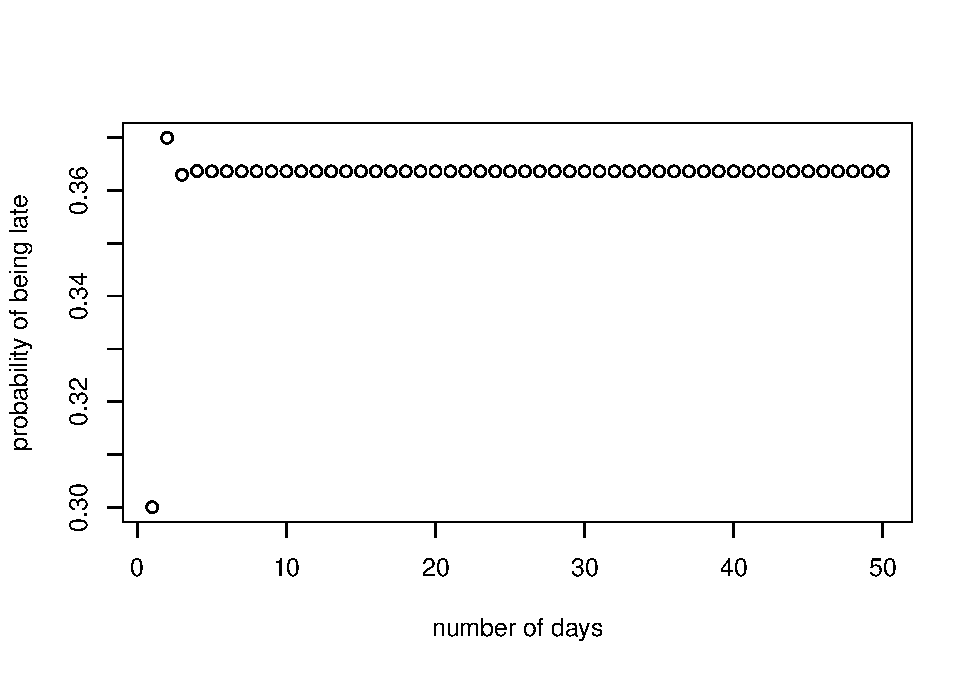
\includegraphics[width=0.5\linewidth]{simulating-MC_files/figure-latex/plot_sample_path-1}
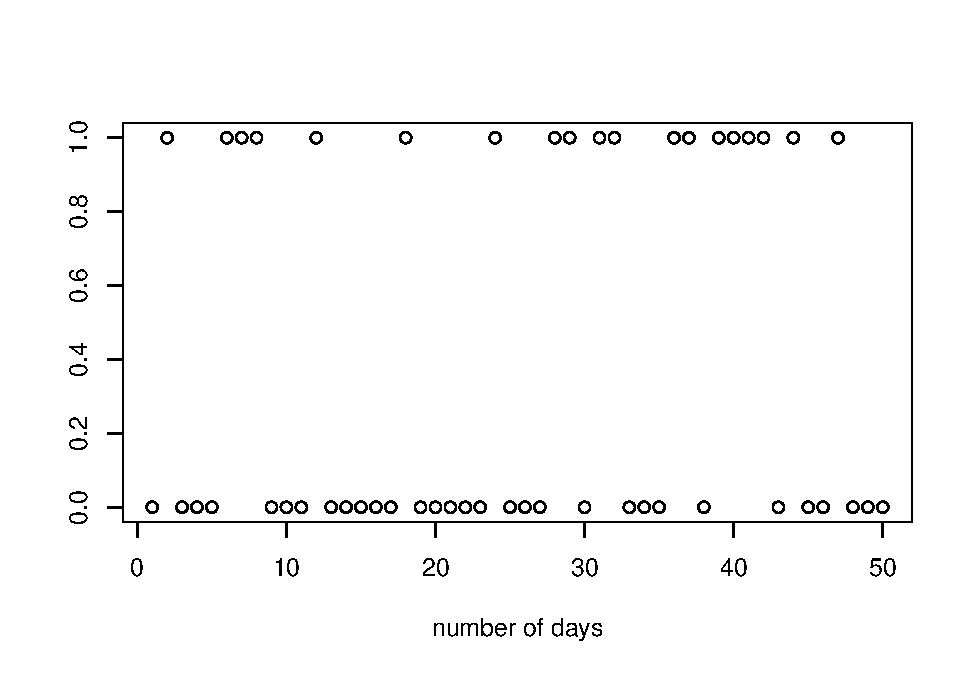
\includegraphics[width=0.5\linewidth]{simulating-MC_files/figure-latex/plot_sample_path-2}

\textbf{Question} If you rerun the above code to simulate a sample path,
you should always get something different. Have a close look at the
figure to the right. The figure on the left will always look very
similar. Why?

\textbf{Question} Rerun the above code to simulate a sample path
changing \(n\), the length of the sample path, and/or the initial value.

\textbf{Question} You can also rerun the whole document using different
transition probabilities. (However, the text might be sometimes
inconsistent\ldots{})


\end{document}
